\begin{center}
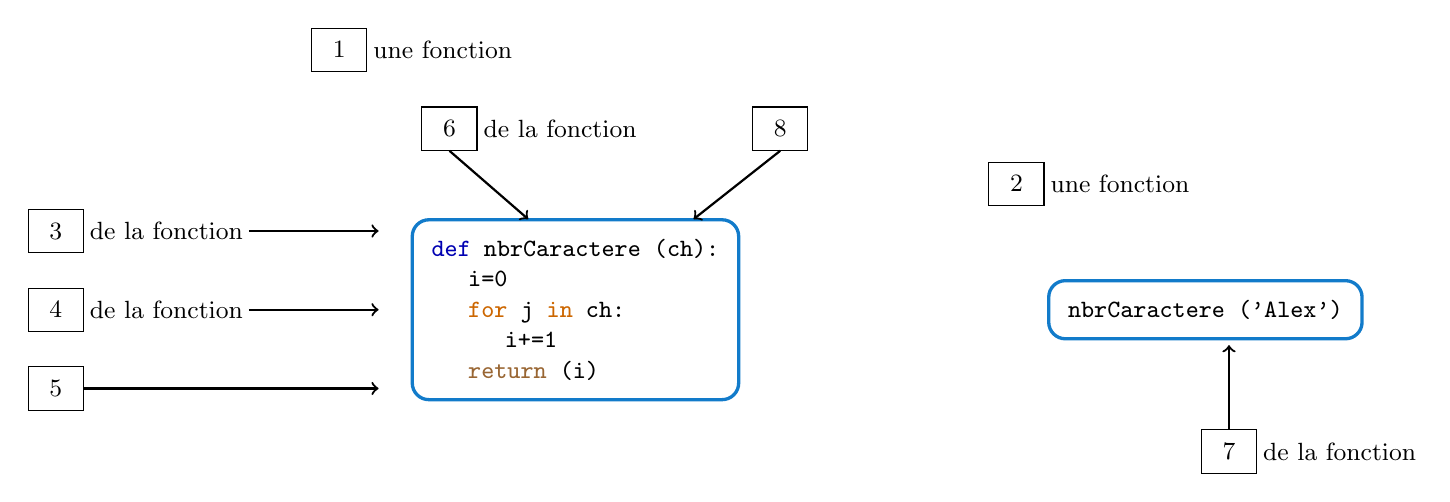
\begin{tikzpicture}[font=\small,
  num/.style={draw,minimum width=0.7cm,minimum height=0.55cm,inner sep=1pt},
  lab/.style={anchor=west,inner sep=2pt},
  box/.style={draw=cyan!60!blue,rounded corners=6pt,very thick,inner sep=7pt}]
\node[box,anchor=center,align=left,font=\ttfamily\small] (g) at (0,0) {%
\textcolor{blue!70!black}{def} nbrCaractere (ch):\\
\hspace*{1.4em}i=0\\
\hspace*{1.4em}\textcolor{orange!80!black}{for} j \textcolor{orange!80!black}{in} ch:\\
\hspace*{2.8em}i+=1\\
\hspace*{1.4em}\textcolor{brown!80!black}{return} (i)};
\node[box,font=\ttfamily\small] (d) at (8,0) {nbrCaractere ('Alex')};
\node[num] (n1) at (-3,3.3) {1}; \node[lab] at (n1.east) {une fonction};
\node[num] (n2) at (5.6,1.6) {2}; \node[lab] at (n2.east) {une fonction};
\node[num] (n6) at (-1.6,2.3) {6}; \node[lab] at (n6.east) {de la fonction};
\node[num] (n8) at (2.6,2.3) {8};
\node[num] (n3) at (-6.6,1.0) {3}; \node[lab] (t3) at (n3.east) {de la fonction};
\node[num] (n4) at (-6.6,0) {4}; \node[lab] (t4) at (n4.east) {de la fonction};
\node[num] (n5) at (-6.6,-1.0) {5};
\node[num] (n7) at (8.3,-1.8) {7}; \node[lab] at (n7.east) {de la fonction};
\draw[->,thick] (t3.east) -- (-2.5,1.0);
\draw[->,thick] (t4.east) -- (-2.5,0);
\draw[->,thick] (n5.east) -- (-2.5,-1.0);
\draw[->,thick] (n6.south) -- (-0.6,1.15);
\draw[->,thick] (n8.south) -- (1.5,1.15);
\draw[->,thick] (n7.north) -- (8.3,-0.45);
\end{tikzpicture}
\end{center}
